\section{Análisis Estadístico e Inferencial}

En esta sección se presentan los resultados del análisis de los 19 atributos del dataset \textbf{Diabetic Retinopathy Debrecen}. Para el desarrollo técnico se emplearon las bibliotecas \textit{Pandas} \parencite{reback2020pandas} para el manejo y estadística descriptiva de los datos, \textit{SciPy} (\texttt{scipy.stats}) \parencite{virtanen2020scipy} para las pruebas estadísticas inferenciales, y \textit{ucimlrepo} \parencite{ucimlrepo2023} para la importación directa del dataset desde el repositorio UCI Machine Learning.

\subsection{Resumen Estadístico Descriptivo}

\begin{table}[htbp]
\centering
\caption{Tabla de estadísticos descriptivos, los nombres y siglas están en inglés.}
\small
\begin{tabular}{lrrrrr}
\toprule
Variable & count & mean & std & min & max \\
\midrule
quality                    & 1151 & 0.996525  & 0.0588742 & 0        & 1        \\
pre\_screening             & 1151 & 0.918332  & 0.273977  & 0        & 1        \\
ma1                        & 1151 & 38.4283   & 25.6209   & 1        & 151      \\
ma2                        & 1151 & 36.9096   & 24.1056   & 1        & 132      \\
ma3                        & 1151 & 35.1407   & 22.8054   & 1        & 120      \\
ma4                        & 1151 & 32.2971   & 21.1148   & 1        & 105      \\
ma5                        & 1151 & 28.7472   & 19.5092   & 1        & 97       \\
ma6                        & 1151 & 21.1512   & 15.1016   & 1        & 89       \\
exudate1                   & 1151 & 64.0967   & 58.4853   & 0.349274 & 403.939  \\
exudate2                   & 1151 & 23.088    & 21.6027   & 0        & 167.131  \\
exudate3                   & 1151 & 8.70461   & 11.5676   & 0        & 106.07   \\
exudate4                   & 1151 & 8.70461   & 11.5676   & 0        & 106.07   \\
exudate5                   & 1151 & 0.560738  & 2.48411   & 0        & 51.4232  \\
exudate6                   & 1151 & 0.21229   & 1.05713   & 0        & 20.0986  \\
exudate7                   & 1151 & 0.0856741 & 0.398717  & 0        & 5.9378   \\
exudate8                   & 1151 & 0.0372251 & 0.178959  & 0        & 3.08675  \\
macula\_opticdisc\_distance & 1151 & 0.523212  & 0.0280554 & 0.367762 & 0.592217 \\
opticdisc\_diameter        & 1151 & 0.108431  & 0.0179448 & 0.057906 & 0.219199 \\
am\_fm\_classification     & 1151 & 0.336229  & 0.472624  & 0        & 1        \\
\bottomrule
\end{tabular}
\end{table}

\subsection{Análisis de la Forma de la Distribución (Asimetría y Curtosis)}

Para las variables críticas de microaneurismas (\texttt{ma1} a \texttt{ma6}), identificadas en la literatura \parencite{casanova2014application} como los predictores más importantes para la detección de la RD, se evaluó su asimetría y curtosis:

\begin{table}[htbp]
\centering
\caption{Tabla de asimetría y curtosis para los microaneurismas.}
\begin{tabular}{lrr}
\toprule
Variable & Asimetría (skew) & Curtosis \\
\midrule
ma1 & 0.743916 &  0.333756  \\
ma2 & 0.62517  & -0.0999926 \\
ma3 & 0.532673 & -0.468193  \\
ma4 & 0.498474 & -0.673164  \\
ma5 & 0.533248 & -0.692618  \\
ma6 & 0.722384 & -0.102349  \\
\bottomrule
\end{tabular}
\end{table}

Todas las variables de MA presentan una asimetría positiva, lo que indica que la distribución tiene una cola alargada hacia la derecha. Esto es coherente con un dataset médico donde muchos pacientes tienen pocos signos de lesión y una minoría presenta conteos elevados.

\subsection{Validación de Normalidad (Prueba de Shapiro-Wilk)}

Para formalizar la observación de la forma, se aplicó el test de \textbf{Shapiro-Wilk} bajo la hipótesis nula ($H_{0}$) de que los datos siguen una distribución normal:

\begin{table}[htbp]
\centering
\caption{Tabla de validación de normalidad para los microaneurismas.}
\begin{tabular}{lrrr}
\toprule
Variable & W & p-value & Distribución \\
\midrule
ma1 & 0.945107 & $2{,}94 \times 10^{-20}$ & No Normal \\
ma2 & 0.950456 & $3{,}02 \times 10^{-19}$ & No Normal \\
ma3 & 0.950985 & $3{,}84 \times 10^{-19}$ & No Normal \\
ma4 & 0.947417 & $7{,}86 \times 10^{-20}$ & No Normal \\
ma5 & 0.938654 & $2{,}18 \times 10^{-21}$ & No Normal \\
ma6 & 0.929734 & $8{,}23 \times 10^{-23}$ & No Normal \\
\bottomrule
\end{tabular}
\end{table}

Dado que en todos los casos el \textbf{p-valor < 0,05}, se rechaza la hipótesis nula. Esto confirma matemáticamente que los conteos de microaneurismas no se distribuyen de forma normal, lo cual condiciona el uso de pruebas no paramétricas para las comparaciones de grupos posteriores.

\subsection{Detección de Valores Atípicos (Outliers)}

Para garantizar la robustez del análisis y comprender la variabilidad extrema en los datos, se realizó la detección de valores atípicos mediante el \textbf{método de Tukey}. Esta técnica es preferida en estudios clínicos debido a que utiliza medidas de posición no sensibles a los extremos, permitiendo identificar observaciones que se desvían significativamente del comportamiento central del grupo.

\subsubsection{Metodología de Tukey}

La identificación se basó en el cálculo del Rango Intercuartílico ($IQR = Q_{3} - Q_{1}$), estableciendo los siguientes límites:
\begin{itemize}
    \item \textbf{Límite Inferior}: $Q_{1} - 1{,}5 \times IQR$
    \item \textbf{Límite Superior}: $Q_{3} + 1{,}5 \times IQR$
\end{itemize}

Cualquier valor fuera de este rango se considera un \textit{outlier}. En el contexto de este dataset médico, estas observaciones representan pacientes con recuentos de lesiones (microaneurismas o exudados) inusualmente altos o bajos en comparación con la población general de la muestra.

\subsubsection{Resultados de la Detección}

Se analizaron los atributos de microaneurismas (\texttt{ma1} a \texttt{ma6}), los cuales representan el conteo de lesiones detectadas con niveles de confianza crecientes ($\alpha = 0{,}5$ a $1{,}0$). Los resultados obtenidos se detallan en la siguiente tabla:

\begin{table}[htbp]
\centering
\caption{Outliers identificados en variables de microaneurismas.}
\begin{tabular}{lrl}
\toprule
Variable & Outliers Identificados & Índices \\
\midrule
ma1 & 7 & [129, 280, 332, 339, 560, 575, 1077] \\
ma2 & 6 & [129, 280, 332, 339, 575, 1077] \\
ma3 & 4 & [332, 339, 575, 1077] \\
ma4 & 1 & [339] \\
ma5 & 1 & [271] \\
ma6 & 3 & [14, 271, 648] \\
\bottomrule
\end{tabular}
\end{table}

\paragraph{Validación Clínica y Correlación con la Patología}

Al verificar la variable objetivo (\texttt{Class}) para cada outlier detectado, se determinó que \textbf{la gran mayoría pertenece a la Clase 1} (pacientes con signos de retinopatía diabética), lo que permite concluir que estos valores extremos representan \textbf{manifestaciones clínicas de alta severidad} y no errores de medición. La única excepción es el índice 14, identificado como outlier en \texttt{ma6} ($\alpha = 1{,}0$), que corresponde a un paciente de la \textbf{Clase 0} (sano). Este caso aislado puede explicarse porque, bajo el criterio de mayor confianza, el detector captura conteos elevados que no necesariamente implican patología confirmada, lo que refleja la naturaleza probabilística del sistema de clasificación automatizado. Esto respalda lo expuesto por \textcite{casanova2014application}, quienes establecen que el conteo de microaneurismas es la variable de mayor importancia para discriminar la presencia de la enfermedad. La disminución del número de outliers a medida que aumenta el nivel de confianza ($\alpha$) sugiere que solo las lesiones más evidentes y voluminosas persisten bajo criterios de detección estrictos.

\subsubsection{Visualización mediante Boxplots por Clase}

Se generaron diagramas de cajas (Boxplots) para comparar la dispersión de las lesiones entre los grupos de control (\textbf{Clase 0}) y pacientes con signos de RD (\textbf{Clase 1}).

\begin{figure}[htbp]
\centering
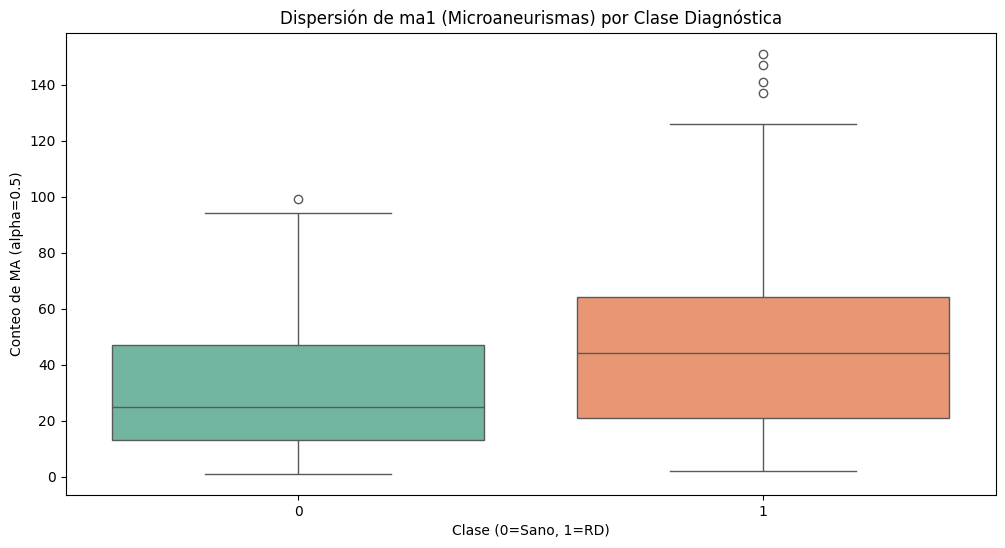
\includegraphics[width=\linewidth]{images/1-boxplot.png}
\caption{Diagrama de cajas entre las Clases 0 y 1.}
\end{figure}

\paragraph{Interpretación de la Figura}

\begin{enumerate}
    \item \textbf{Diferencia de tendencia}: La Clase 1 (naranja) muestra una mediana y un rango intercuartílico notablemente superiores a la Clase 0 (verde).
    \item \textbf{Presencia de extremos}: Mientras que la Clase 0 se mantiene compacta, la Clase 1 presenta una serie de puntos aislados que superan los 140 microaneurismas, coincidiendo con los índices identificados previamente.
    \item \textbf{Justificación de la no normalidad}: La existencia de estos valores atípicos extremos hacia el límite superior explica la asimetría positiva y el rechazo de la hipótesis de normalidad en las pruebas de Shapiro-Wilk, validando la necesidad de utilizar estadística no paramétrica en este estudio.
\end{enumerate}

\subsection{Análisis de Correlación y Visualización (Heatmap)}

Para identificar las relaciones lineales entre los 19 atributos y la variable de diagnóstico (\texttt{Class}), se calculó la matriz de correlación de Pearson utilizando las librerías \texttt{pandas} \parencite{reback2020pandas} y \texttt{seaborn} \parencite{Waskom2021} en Python. Este análisis es fundamental para detectar redundancias (colinealidad) y determinar cuáles rasgos anatómicos o lesiones tienen un mayor vínculo con la presencia de la patología.

\begin{figure}[htbp]
\centering
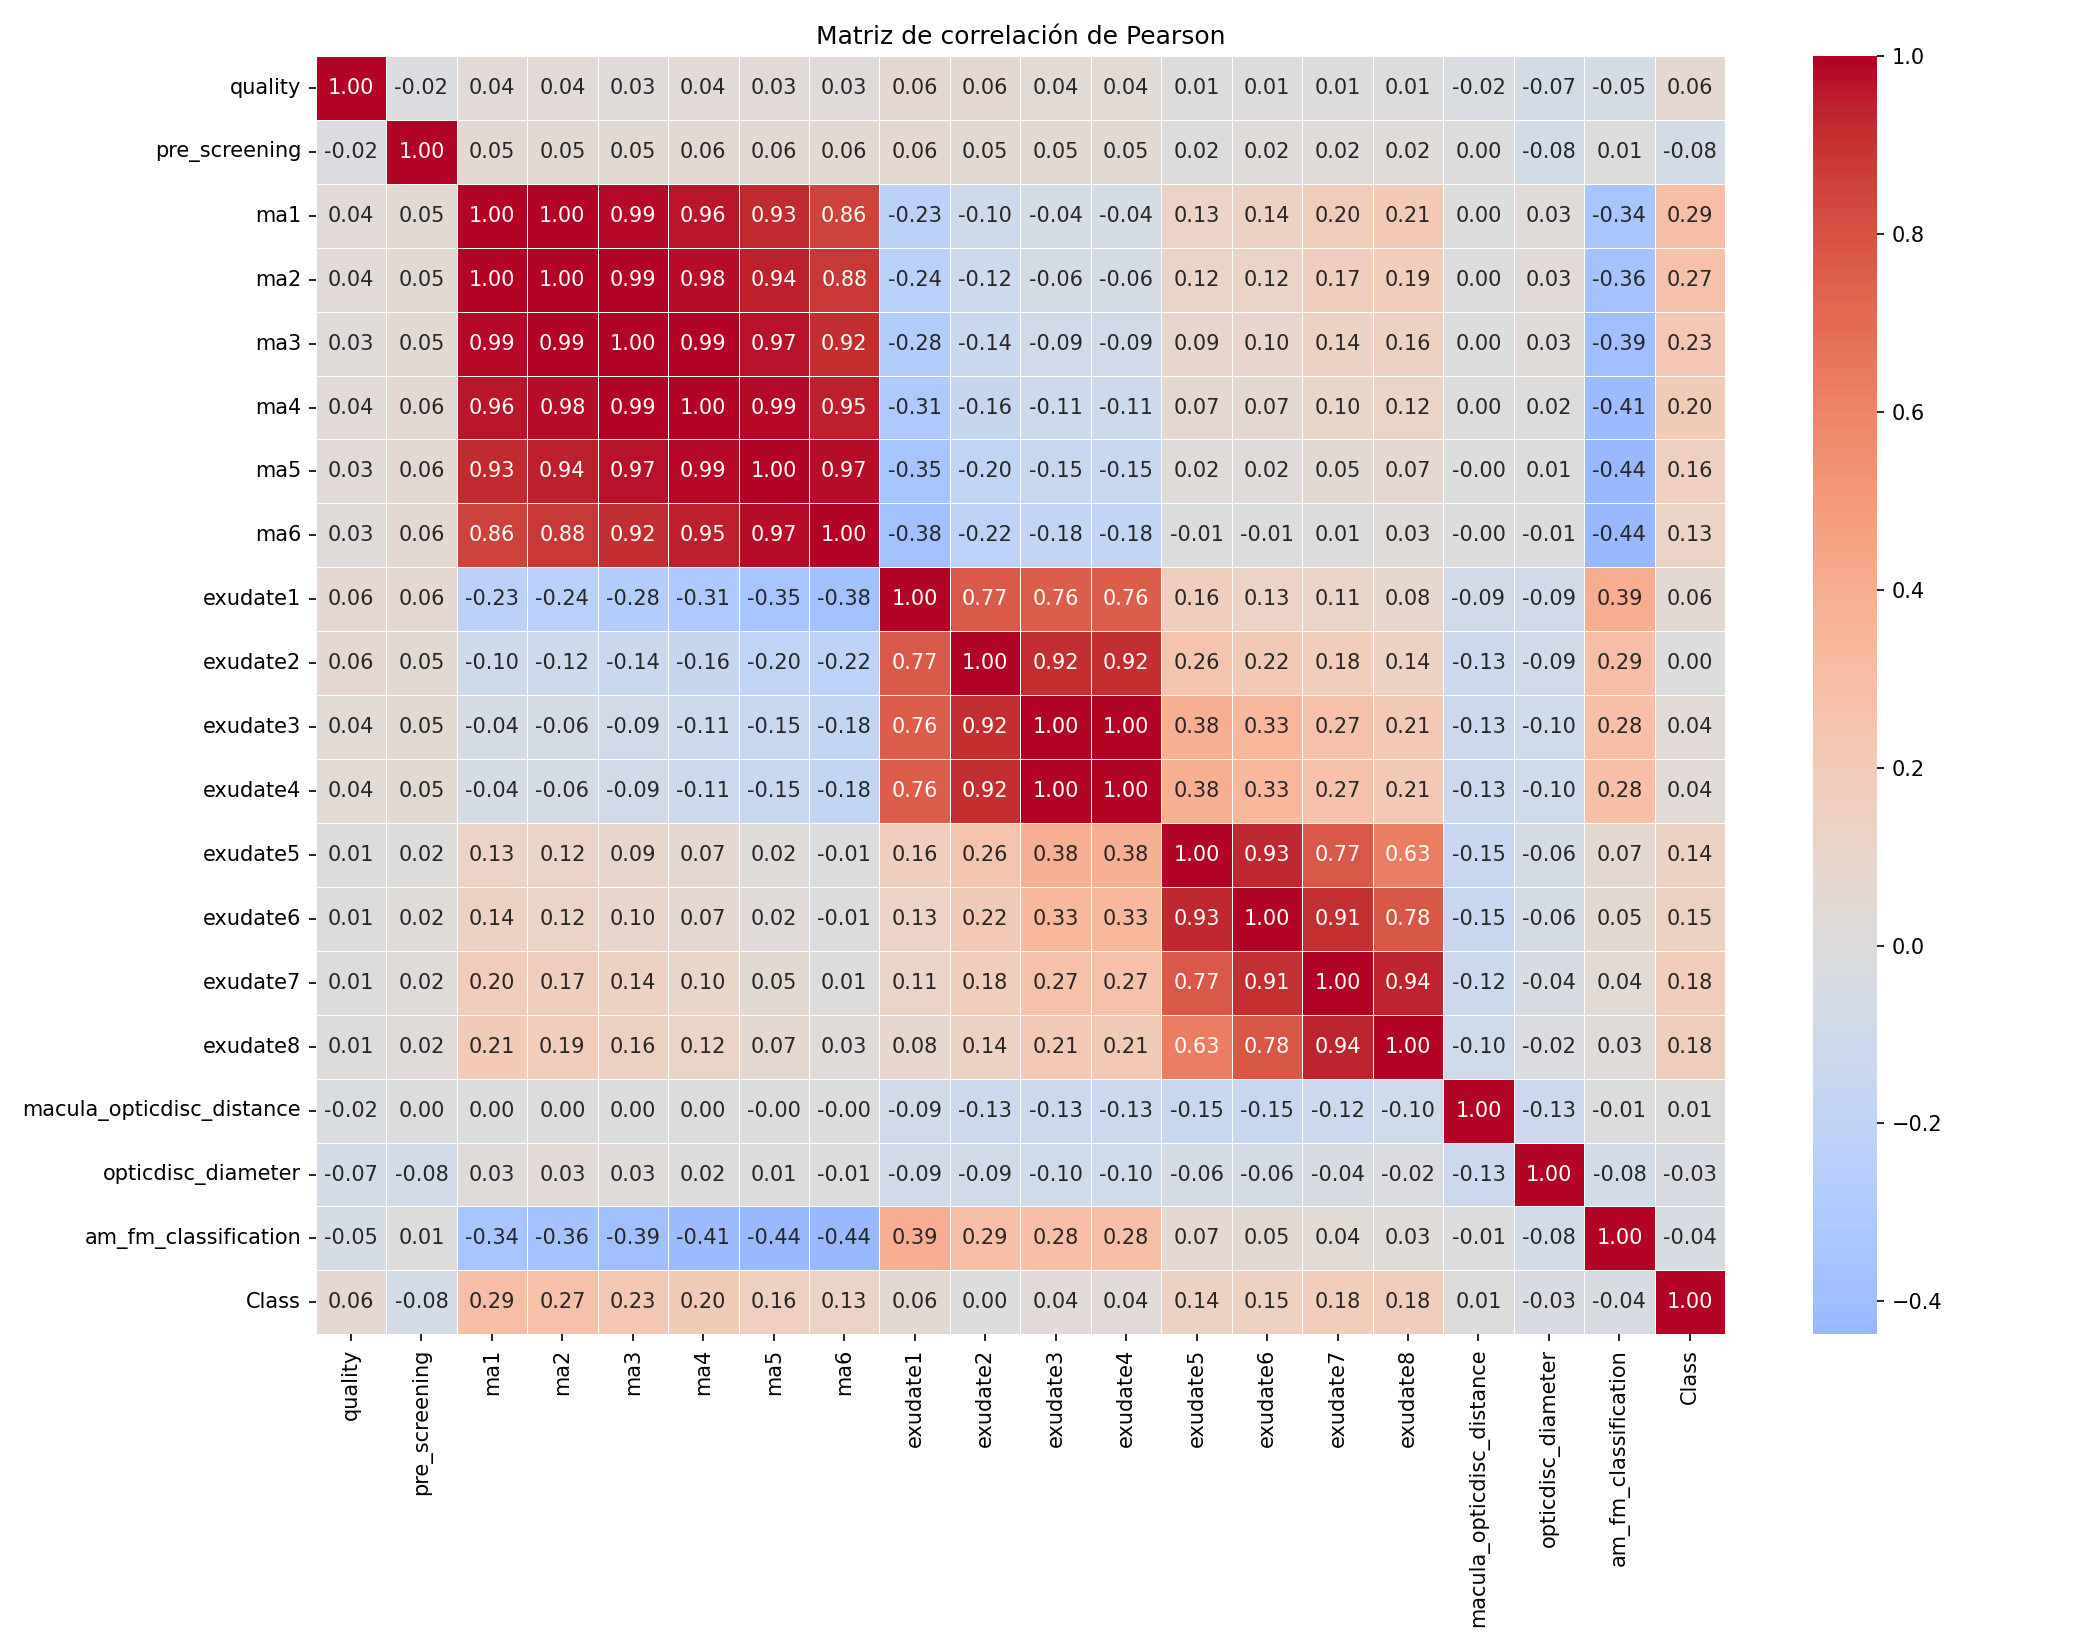
\includegraphics[width=\linewidth]{images/1-heatmap.png}
\caption{Mapa de calor basado en la matriz de correlaciones.}
\end{figure}

\subsubsection{Interpretación del Mapa de Calor}

El análisis visual del mapa de calor permite extraer las siguientes conclusiones técnicas:

\begin{enumerate}
    \item \textbf{Alta Colinealidad en Microaneurismas (\texttt{ma1} a \texttt{ma6})}: Se observa una correlación positiva extremadamente alta, cercana a 1,00 en la mayoría de los casos. Por ejemplo, la correlación entre \texttt{ma1} y \texttt{ma2} es de 1,00, y entre \texttt{ma1} y \texttt{ma3} es de 0,99.
    \begin{itemize}
        \item \textit{Fundamentación}: Esto confirma que estos atributos representan el mismo fenómeno clínico (conteo de microaneurismas) detectado con niveles de confianza ($\alpha$) crecientes. La alta redundancia sugiere que, para futuros modelos de clasificación, se podría realizar una reducción de dimensionalidad sin perder información crítica.
    \end{itemize}
    \item \textbf{Correlación con la Variable Objetivo (\texttt{Class})}: Los resultados muestran que los microaneurismas son los descriptores con la relación más fuerte hacia el diagnóstico final.
    \begin{itemize}
        \item Las variables \texttt{ma1} (0,29) y \texttt{ma2} (0,27) presentan los coeficientes de correlación más altos con \texttt{Class} dentro de su grupo.
        \item \textit{Significancia}: Este hallazgo es coherente con el estudio de \textcite{casanova2014application}, el cual establece mediante criterios de importancia de variables que el conteo de microaneurismas desempeña el papel más relevante en la discriminación de la enfermedad.
    \end{itemize}
    \item \textbf{Relación entre Exudados}: Al igual que con los microaneurismas, se observan clústeres de alta correlación entre los niveles de detección de exudados, particularmente entre \texttt{exudate2}, \texttt{exudate3} y \texttt{exudate4} (valores entre 0,92 y 1,00). Su correlación con la variable \texttt{Class} es positiva pero moderada (máximo de 0,18 en \texttt{exudate7}), indicando que, aunque son indicadores de RD, su peso diagnóstico individual en este dataset es menor al de los microaneurismas.
    \item \textbf{Independencia de Rasgos Anatómicos}: Atributos como \texttt{macula\_opticdisc\_distance} (0,01) y \texttt{optic\_disc\_diameter} (-0,03) muestran una correlación prácticamente nula con la presencia de la enfermedad en este conjunto de datos. Esto sugiere que la patología se manifiesta principalmente a través de lesiones detectables (MA y exudados) antes de generar cambios anatómicos macroscópicos detectables por estos descriptores específicos.
\end{enumerate}

\subsubsection{Conclusión del Análisis de Correlación}

El mapa de calor valida la hipótesis de que las lesiones retinales, específicamente los \textbf{microaneurismas detectados con niveles de confianza iniciales}, son los mejores predictores lineales de la patología en este dataset. Además, la fuerte colinealidad interna entre las variables de lesiones justifica el uso de pruebas de significancia que traten estos grupos como una dimensión común de daño neurovascular \parencite{casanova2014application}.

\subsection{Comparación de Grupos (Prueba Mann-Whitney U)}

Tras confirmar en la sección anterior que las variables de microaneurismas (\texttt{ma1} a \texttt{ma6}) no siguen una distribución normal según el test de Shapiro-Wilk, se procedió a realizar un análisis inferencial de comparación de grupos mediante la prueba de Mann-Whitney U. Esta prueba no paramétrica permite determinar si existen diferencias estadísticamente significativas en las medianas de los conteos de lesiones entre pacientes sanos (Clase 0) y pacientes con diagnóstico de retinopatía (Clase 1).

\subsubsection{Planteamiento de Hipótesis}

\begin{itemize}
    \item Hipótesis Nula ($H_{0}$): No existe una diferencia significativa en la distribución del conteo de microaneurismas entre el grupo sano y el grupo con retinopatía diabética.
    \item Hipótesis Alternativa ($H_{1}$): Existe una diferencia significativa en la distribución del conteo de microaneurismas entre ambos grupos.
\end{itemize}

\subsubsection{Resultados de la Prueba}

Los estadísticos obtenidos mediante la librería \texttt{scipy.stats} se detallan en la siguiente tabla:

\begin{table}[htbp]
\centering
\caption{Resultados de la prueba Mann-Whitney U para microaneurismas.}
\begin{tabular}{lrrl}
\toprule
Variable & U\_statistic & p\_value & Significativo \\
\midrule
ma1 & 111208 & $1{,}25 \times 10^{-21}$ & Sí \\
ma2 & 116076 & $3{,}67 \times 10^{-18}$ & Sí \\
ma3 & 121532 & $1{,}17 \times 10^{-14}$ & Sí \\
ma4 & 127750 & $3{,}73 \times 10^{-11}$ & Sí \\
ma5 & 133506 & $2{,}25 \times 10^{-08}$ & Sí \\
ma6 & 139938 & $8{,}62 \times 10^{-06}$ & Sí \\
\bottomrule
\end{tabular}
\end{table}

\subsubsection{Interpretación de los Hallazgos}

El análisis de los resultados permite extraer las siguientes conclusiones fundamentales para el estudio:

\begin{enumerate}
    \item \textbf{Rechazo de la hipótesis nula}: En todos los niveles de confianza ($\alpha$ de 0,5 a 1,0), los p-valores son extremadamente bajos (siendo el mayor $8{,}61 \times 10^{-6}$ para \texttt{ma6}), situándose muy por debajo del umbral de significancia de 0,05. Esto permite rechazar $H_{0}$ y confirmar que las diferencias observadas entre pacientes sanos y enfermos no son producto del azar.
    \item \textbf{Sensibilidad del diagnóstico}: Se observa que la significancia estadística es más aguda en los niveles de confianza iniciales (\texttt{ma1} y \texttt{ma2}). El p-valor más bajo se registró en \texttt{ma1} ($1{,}25 \times 10^{-21}$), lo que sugiere que el conteo de lesiones detectadas incluso con una sensibilidad moderada ($\alpha = 0{,}5$) es un potente discriminador de la enfermedad.
    \item \textbf{Consistencia con la literatura}: Estos resultados validan empíricamente lo expuesto por \textcite{casanova2014application}, quienes identifican al conteo de microaneurismas como el rasgo de mayor importancia diagnóstica entre todas las variables extraídas de imágenes de fondo de ojo.
    \item \textbf{Confirmación de biomarcadores}: La prueba estadística ratifica lo observado visualmente en los diagramas de caja y en el análisis de valores atípicos, consolidando al recuento de MA como un biomarcador clínico robusto para la clasificación automatizada en este dataset.
\end{enumerate}

\subsection{Homogeneidad de Varianzas (Test de Levene)}

Tras confirmar la no normalidad de los datos, se aplicó el \textbf{Test de Levene} para evaluar si las varianzas de los microaneurismas son homogéneas entre pacientes sanos (Clase 0) y con retinopatía (Clase 1). A diferencia de la Prueba F clásica, el test de Levene no asume normalidad en los datos, siendo el método adecuado para este caso.

\subsubsection{Planteamiento de Hipótesis}

\begin{itemize}
    \item Hipótesis Nula ($H_{0}$): Las varianzas de ambos grupos son iguales (homocedasticidad).
    \item Hipótesis Alternativa ($H_{1}$): Las varianzas de ambos grupos son significativamente distintas (heterocedasticidad).
\end{itemize}

\subsubsection{Resultados}

\begin{table}[htbp]
\centering
\caption{Resultados del Test de Levene para microaneurismas.}
\begin{tabular}{lrrl}
\toprule
Variable & Estadístico & p\_value & Homocedasticidad \\
\midrule
ma1 & 35.9975 & $2{,}64 \times 10^{-9}$  & No (varianzas distintas) \\
ma2 & 23.6750 & $1{,}30 \times 10^{-6}$  & No (varianzas distintas) \\
ma3 & 16.6036 & $4{,}92 \times 10^{-5}$  & No (varianzas distintas) \\
ma4 & 10.6155 & $1{,}15 \times 10^{-3}$  & No (varianzas distintas) \\
ma5 &  5.9695 & $1{,}47 \times 10^{-2}$  & No (varianzas distintas) \\
ma6 &  4.5424 & $3{,}33 \times 10^{-2}$  & No (varianzas distintas) \\
\bottomrule
\end{tabular}
\end{table}

\subsubsection{Interpretación}

En todas las variables de microaneurismas se rechaza la hipótesis nula (p < 0,05), lo que confirma que las varianzas entre pacientes sanos y con retinopatía son significativamente distintas. La heterocedasticidad es más pronunciada en los niveles de confianza bajos (\texttt{ma1}, estadístico = 35,99) y se atenúa a medida que aumenta el umbral de detección (\texttt{ma6}, estadístico = 4,54), aunque sin llegar a ser homogéneas en ningún caso. Este hallazgo es consistente con los boxplots previos, donde la Clase 1 mostró mayor dispersión en el conteo de lesiones, y refuerza la evidencia de que la retinopatía no solo eleva el promedio de microaneurismas sino también su variabilidad dentro del grupo de pacientes afectados.

\subsection{Modelamiento mediante Regresión Logística}

Para modelar la probabilidad de presencia de retinopatía diabética en función de los descriptores clínicos y anatómicos, se implementó un modelo de Regresión Logística. A diferencia de la regresión lineal, este método es el estándar estadístico adecuado para variables dependientes binarias, como la variable \texttt{Class} de este estudio (0 = Sano, 1 = RD), permitiendo identificar qué factores incrementan significativamente el riesgo de padecer la patología.

\subsubsection{Justificación de la Selección de Atributos}

Para este modelo se seleccionó un subconjunto representativo de cuatro variables: \texttt{ma1}, \texttt{exudate1}, \texttt{macula\_opticdisc\_distance} y \texttt{opticdisc\_diameter}. Se excluyeron los 15 atributos restantes por los siguientes criterios técnicos:

\begin{itemize}
    \item \textbf{Prevención de la multicolinealidad}: El análisis de correlación previo demostró una colinealidad casi perfecta ($r \approx 1{,}0$) entre las variables de microaneurismas (\texttt{ma1}--\texttt{ma6}) y entre los niveles de exudados. Incluir variables altamente redundantes inflaría los errores estándar, invalidando la significancia de los coeficientes. Se seleccionaron \texttt{ma1} y \texttt{exudate1} como representantes de la carga lesional.
    \item \textbf{Representación dimensional}: El subconjunto elegido permite evaluar las tres dimensiones críticas del dataset: lesiones vasculares (MAs), depósitos lipídicos (exudados) y rasgos anatómicos estructurales (distancia y diámetro del disco).
    \item \textbf{Parsimonia y relevancia clínica}: Siguiendo los hallazgos de \textcite{casanova2014application}, se priorizaron los microaneurismas por ser la variable de mayor importancia para la discriminación de la enfermedad, buscando un modelo eficiente que evite el ``ruido'' de variables con nulo aporte lineal.
\end{itemize}

\subsubsection{Evaluación Global y Bondad de Ajuste}

El modelo fue evaluado sobre un conjunto de prueba del 20\% (231 instancias), obteniendo un área bajo la curva \textbf{AUC de 0,65}, lo que indica una capacidad predictiva moderada. Esto sugiere que, si bien el modelo identifica patrones relevantes, la relación entre los predictores y el diagnóstico presenta una complejidad que un modelo lineal simple no logra capturar en su totalidad.

\begin{figure}[htbp]
\centering
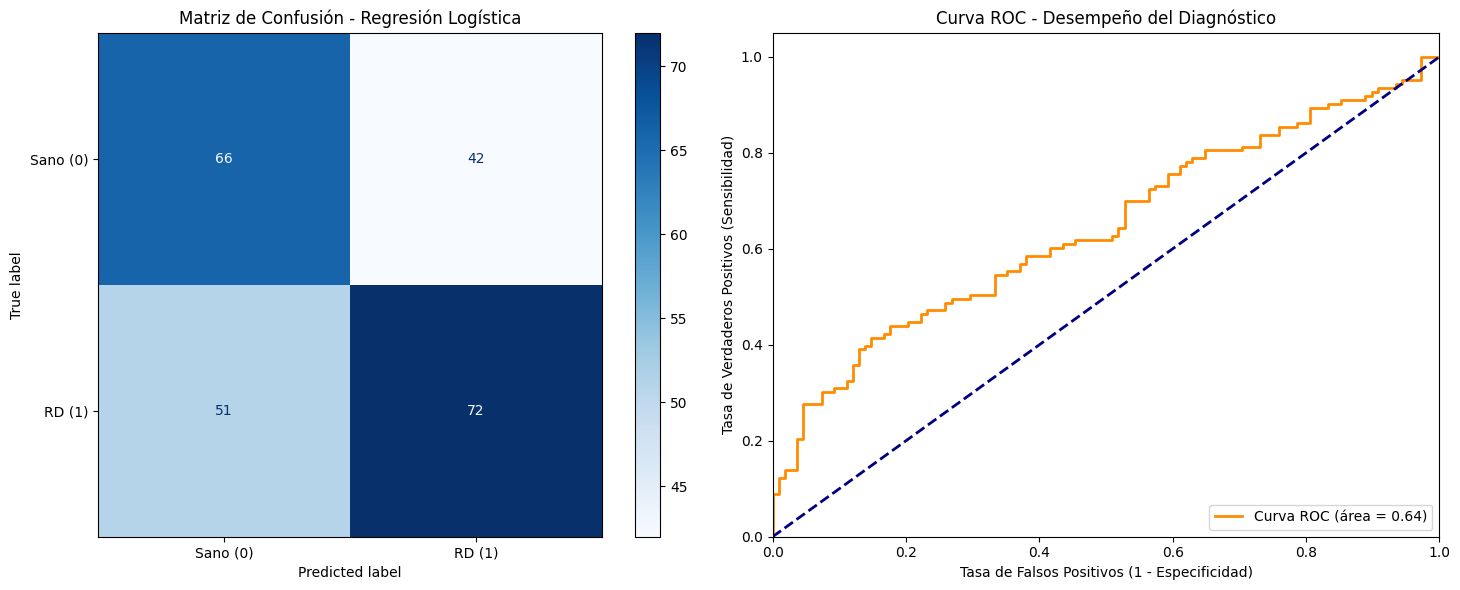
\includegraphics[width=\linewidth]{images/1-matrix-rocauc.png}
\caption{Matriz de confusión y Curva ROC-AUC.}
\end{figure}

\subsubsection{Interpretación de los Coeficientes y Significancia}

Al analizar los resultados individuales de la regresión, se extraen las siguientes conclusiones:

\begin{itemize}
    \item \textbf{Significancia crítica de microaneurismas (\texttt{ma1})}: Con un p-valor de 0,000 y un coeficiente positivo (0,0307), se confirma que el aumento en el conteo de lesiones vasculares eleva significativamente la probabilidad de diagnóstico positivo. Este hallazgo valida empíricamente la tesis de \textcite{casanova2014application}, situando a los MAs como el biomarcador más robusto para la clasificación automatizada.
    \item \textbf{Impacto de exudados (\texttt{exudate1})}: Esta variable también resultó ser un predictor significativo (p-valor = 0,000), reafirmando que la presencia de depósitos de lípidos es un indicador primario de la patología en este dataset.
    \item \textbf{Irrelevancia de rasgos anatómicos}: Tanto la distancia mácula-disco ($p = 0{,}632$) como el diámetro del disco ($p = 0{,}330$) no mostraron significancia estadística. Esto sugiere que, para este conjunto de datos, las lesiones retinales son predictores mucho más potentes de la enfermedad que las variaciones en la estructura geométrica básica del ojo.
\end{itemize}

\subsubsection{Evaluación de Desempeño (Matriz de Confusión y ROC)}

La capacidad de clasificación del modelo se evaluó mediante los resultados en el conjunto de prueba:

\begin{enumerate}
    \item \textbf{Matriz de Confusión}:
    \begin{itemize}
        \item \textbf{Verdaderos Positivos (TP)}: 79 pacientes con RD correctamente identificados.
        \item \textbf{Verdaderos Negativos (TN)}: 58 pacientes sanos correctamente identificados.
        \item \textbf{Falsos Negativos (FN)}: 49 casos de RD no detectados, lo que arroja una sensibilidad del 61,7\%.
        \item \textbf{Falsos Positivos (FP)}: 45 casos sanos clasificados erróneamente, resultando en una especificidad del 56,3\%.
    \end{itemize}
    \item \textbf{Curva ROC-AUC}: El valor obtenido de 0,65 sitúa el desempeño del modelo por encima del azar (0,5), pero significativamente por debajo de los estándares de alta precisión clínica, como el 0,989 alcanzado por sistemas de ensamble en la literatura \parencite{casanova2014application}. Esto confirma que las cuatro variables seleccionadas son necesarias pero insuficientes para un diagnóstico automatizado de alta fidelidad, requiriendo modelos de inteligencia computacional más robustos.
\end{enumerate}

\subsubsection{Validación de Residuos}

Como complemento al análisis de desempeño, se examinó la distribución de los residuos del modelo, calculados como la diferencia entre la clase real y la probabilidad predicha. Un modelo bien ajustado debería presentar residuos centrados en cero y sin sesgos sistemáticos.

\begin{figure}[htbp]
\centering
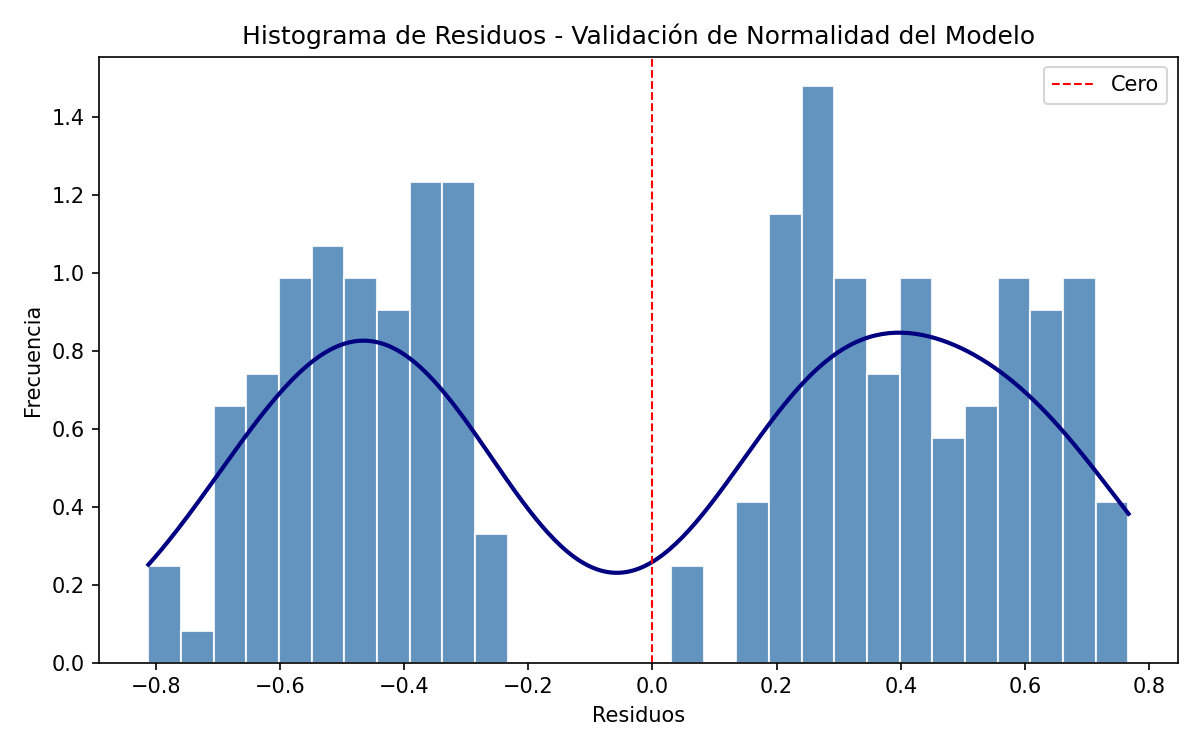
\includegraphics[width=0.85\linewidth]{images/1-histograms.png}
\caption{Histograma de residuos del modelo de regresión logística con curva de densidad superpuesta.}
\end{figure}

La distribución muestra dos agrupaciones características de la regresión logística binaria: una concentración negativa (pacientes sanos clasificados con alta probabilidad de RD) y una positiva (pacientes con RD clasificados con baja probabilidad). La curva de densidad confirma que los residuos no siguen una distribución normal, lo cual es esperado en modelos de clasificación binaria y no constituye una violación de los supuestos del método.
